\documentclass[]{book}
\usepackage{lmodern}
\usepackage{amssymb,amsmath}
\usepackage{ifxetex,ifluatex}
\usepackage{fixltx2e} % provides \textsubscript
\ifnum 0\ifxetex 1\fi\ifluatex 1\fi=0 % if pdftex
  \usepackage[T1]{fontenc}
  \usepackage[utf8]{inputenc}
\else % if luatex or xelatex
  \ifxetex
    \usepackage{mathspec}
  \else
    \usepackage{fontspec}
  \fi
  \defaultfontfeatures{Ligatures=TeX,Scale=MatchLowercase}
\fi
% use upquote if available, for straight quotes in verbatim environments
\IfFileExists{upquote.sty}{\usepackage{upquote}}{}
% use microtype if available
\IfFileExists{microtype.sty}{%
\usepackage{microtype}
\UseMicrotypeSet[protrusion]{basicmath} % disable protrusion for tt fonts
}{}
\usepackage[margin=1in]{geometry}
\usepackage{hyperref}
\hypersetup{unicode=true,
            pdftitle={ND111 - Data Science II - Notebook},
            pdfborder={0 0 0},
            breaklinks=true}
\urlstyle{same}  % don't use monospace font for urls
\usepackage{natbib}
\bibliographystyle{apalike}
\usepackage{color}
\usepackage{fancyvrb}
\newcommand{\VerbBar}{|}
\newcommand{\VERB}{\Verb[commandchars=\\\{\}]}
\DefineVerbatimEnvironment{Highlighting}{Verbatim}{commandchars=\\\{\}}
% Add ',fontsize=\small' for more characters per line
\usepackage{framed}
\definecolor{shadecolor}{RGB}{248,248,248}
\newenvironment{Shaded}{\begin{snugshade}}{\end{snugshade}}
\newcommand{\KeywordTok}[1]{\textcolor[rgb]{0.13,0.29,0.53}{\textbf{#1}}}
\newcommand{\DataTypeTok}[1]{\textcolor[rgb]{0.13,0.29,0.53}{#1}}
\newcommand{\DecValTok}[1]{\textcolor[rgb]{0.00,0.00,0.81}{#1}}
\newcommand{\BaseNTok}[1]{\textcolor[rgb]{0.00,0.00,0.81}{#1}}
\newcommand{\FloatTok}[1]{\textcolor[rgb]{0.00,0.00,0.81}{#1}}
\newcommand{\ConstantTok}[1]{\textcolor[rgb]{0.00,0.00,0.00}{#1}}
\newcommand{\CharTok}[1]{\textcolor[rgb]{0.31,0.60,0.02}{#1}}
\newcommand{\SpecialCharTok}[1]{\textcolor[rgb]{0.00,0.00,0.00}{#1}}
\newcommand{\StringTok}[1]{\textcolor[rgb]{0.31,0.60,0.02}{#1}}
\newcommand{\VerbatimStringTok}[1]{\textcolor[rgb]{0.31,0.60,0.02}{#1}}
\newcommand{\SpecialStringTok}[1]{\textcolor[rgb]{0.31,0.60,0.02}{#1}}
\newcommand{\ImportTok}[1]{#1}
\newcommand{\CommentTok}[1]{\textcolor[rgb]{0.56,0.35,0.01}{\textit{#1}}}
\newcommand{\DocumentationTok}[1]{\textcolor[rgb]{0.56,0.35,0.01}{\textbf{\textit{#1}}}}
\newcommand{\AnnotationTok}[1]{\textcolor[rgb]{0.56,0.35,0.01}{\textbf{\textit{#1}}}}
\newcommand{\CommentVarTok}[1]{\textcolor[rgb]{0.56,0.35,0.01}{\textbf{\textit{#1}}}}
\newcommand{\OtherTok}[1]{\textcolor[rgb]{0.56,0.35,0.01}{#1}}
\newcommand{\FunctionTok}[1]{\textcolor[rgb]{0.00,0.00,0.00}{#1}}
\newcommand{\VariableTok}[1]{\textcolor[rgb]{0.00,0.00,0.00}{#1}}
\newcommand{\ControlFlowTok}[1]{\textcolor[rgb]{0.13,0.29,0.53}{\textbf{#1}}}
\newcommand{\OperatorTok}[1]{\textcolor[rgb]{0.81,0.36,0.00}{\textbf{#1}}}
\newcommand{\BuiltInTok}[1]{#1}
\newcommand{\ExtensionTok}[1]{#1}
\newcommand{\PreprocessorTok}[1]{\textcolor[rgb]{0.56,0.35,0.01}{\textit{#1}}}
\newcommand{\AttributeTok}[1]{\textcolor[rgb]{0.77,0.63,0.00}{#1}}
\newcommand{\RegionMarkerTok}[1]{#1}
\newcommand{\InformationTok}[1]{\textcolor[rgb]{0.56,0.35,0.01}{\textbf{\textit{#1}}}}
\newcommand{\WarningTok}[1]{\textcolor[rgb]{0.56,0.35,0.01}{\textbf{\textit{#1}}}}
\newcommand{\AlertTok}[1]{\textcolor[rgb]{0.94,0.16,0.16}{#1}}
\newcommand{\ErrorTok}[1]{\textcolor[rgb]{0.64,0.00,0.00}{\textbf{#1}}}
\newcommand{\NormalTok}[1]{#1}
\usepackage{longtable,booktabs}
\usepackage{graphicx,grffile}
\makeatletter
\def\maxwidth{\ifdim\Gin@nat@width>\linewidth\linewidth\else\Gin@nat@width\fi}
\def\maxheight{\ifdim\Gin@nat@height>\textheight\textheight\else\Gin@nat@height\fi}
\makeatother
% Scale images if necessary, so that they will not overflow the page
% margins by default, and it is still possible to overwrite the defaults
% using explicit options in \includegraphics[width, height, ...]{}
\setkeys{Gin}{width=\maxwidth,height=\maxheight,keepaspectratio}
\IfFileExists{parskip.sty}{%
\usepackage{parskip}
}{% else
\setlength{\parindent}{0pt}
\setlength{\parskip}{6pt plus 2pt minus 1pt}
}
\setlength{\emergencystretch}{3em}  % prevent overfull lines
\providecommand{\tightlist}{%
  \setlength{\itemsep}{0pt}\setlength{\parskip}{0pt}}
\setcounter{secnumdepth}{5}
% Redefines (sub)paragraphs to behave more like sections
\ifx\paragraph\undefined\else
\let\oldparagraph\paragraph
\renewcommand{\paragraph}[1]{\oldparagraph{#1}\mbox{}}
\fi
\ifx\subparagraph\undefined\else
\let\oldsubparagraph\subparagraph
\renewcommand{\subparagraph}[1]{\oldsubparagraph{#1}\mbox{}}
\fi

%%% Use protect on footnotes to avoid problems with footnotes in titles
\let\rmarkdownfootnote\footnote%
\def\footnote{\protect\rmarkdownfootnote}

%%% Change title format to be more compact
\usepackage{titling}

% Create subtitle command for use in maketitle
\newcommand{\subtitle}[1]{
  \posttitle{
    \begin{center}\large#1\end{center}
    }
}

\setlength{\droptitle}{-2em}

  \title{ND111 - Data Science II - Notebook}
    \pretitle{\vspace{\droptitle}\centering\huge}
  \posttitle{\par}
    \author{}
    \preauthor{}\postauthor{}
    \date{}
    \predate{}\postdate{}
  
\usepackage{booktabs}

\begin{document}
\maketitle

{
\setcounter{tocdepth}{1}
\tableofcontents
}
\chapter*{Course Info}\label{course-info}
\addcontentsline{toc}{chapter}{Course Info}

Tags

\begin{itemize}
\tightlist
\item
  Author : AH Uyekita
\item
  Dedication : 10 hours/week (suggested)
\item
  Start : 14/12/2018
\item
  End (Planned): 28/12/2018
\item
  Title : Data Science II - Foundations Nanodegree Program

  \begin{itemize}
  \tightlist
  \item
    COD : ND111
  \end{itemize}
\end{itemize}

Related Courses

\begin{itemize}
\tightlist
\item
  \href{https://br.udacity.com/course/python-fundamentos-data-science--nd110}{ND110
  - Data Science I - Nanodegree Foundations}
\end{itemize}

\begin{center}\rule{0.5\linewidth}{\linethickness}\end{center}

Objectives

I want to finish this course in two weeks. It includes the Optional
videos and chapters.

Syllabus

\begin{itemize}
\tightlist
\item
  Chapter 01 - Welcome

  \begin{itemize}
  \tightlist
  \item
    Lesson 01 - Instructions
  \item
    Lesson 02 - Tips
  \end{itemize}
\item
  Chapter 02 - SQL for Data Analysis

  \begin{itemize}
  \tightlist
  \item
    Lesson 01 - Basic SQL
  \item
    Lesson 02 - SQL Joins
  \item
    Lesson 03 - SQL Aggregations
  \item
    Lesson 04 - (Optional) SQL Subqueries \& Temporary Tables (Advanced)
  \item
    Lesson 05 - (Optional) SQL Data Cleaning (Advanced)
  \item
    Project 01 - Query a Digital Music Store Database
  \end{itemize}
\item
  Chapter 03 - Data Wrangling

  \begin{itemize}
  \tightlist
  \item
    Lesson 01 - Introduction to Data Wrangling
  \item
    Lesson 02 - Gathering
  \item
    Lesson 03 - Assessing Data
  \item
    Lesson 04 - Cleaning Data
  \item
    Project 02 - Wrangle and Analyze Data
  \end{itemize}
\item
  Chapter 04 - Advanced Statistics

  \begin{itemize}
  \tightlist
  \item
    Lesson 01 - Descriptive Statistics - Part 1
  \item
    Lesson 02 - Descriptive Statistics - Part 2
  \item
    Lesson 03 - Admissions Case Study
  \item
    Lesson 04 - Probability
  \item
    Lesson 05 - Binomial Distribution
  \item
    Lesson 06 - Conditional Probability
  \item
    Lesson 07 - Bayes Rule
  \item
    Lesson 08 - Python Probability Practice
  \item
    Lesson 09 - Normal Distribution Theory
  \item
    Lesson 10 - Sampling Distributions and the Central Limit Theorem
  \item
    Lesson 11 - Confidence Intervals
  \item
    Lesson 12 - Hypothesis Testing
  \item
    Lesson 13 - Case Study: A/B Tests
  \item
    Lesson 14 - Regression
  \item
    Lesson 15 - Multiple Linear Regression
  \item
    Lesson 16 - Logistic Regression
  \item
    Project 03 - Analyze A/B Test Results
  \end{itemize}
\item
  Chapter 05 - Intro to Machine Learning

  \begin{itemize}
  \tightlist
  \item
    Lesson 01 - Welcome to Machine Learning
  \item
    Lesson 02 - Naive Bayes
  \item
    Lesson 03 - SVM
  \item
    Lesson 04 - Decision Trees
  \item
    Lesson 05 - Choose Your Own Algorithm
  \item
    Lesson 06 - Datasets and Questions
  \item
    Lesson 07 - Regressions
  \item
    Lesson 08 - Outliers
  \item
    Lesson 09 - Clustering
  \item
    Lesson 10 - Feature Scaling
  \item
    Lesson 11 - Text Learning
  \item
    Lesson 12 - Feature Selection
  \item
    Lesson 13 - PCA
  \item
    Lesson 14 - Validation
  \item
    Lesson 15 - Evaluation Metrics
  \item
    Lesson 16 - Tying It All Together
  \item
    Project 04 - Identify Fraud from Enron Email
  \end{itemize}
\item
  Chapter 06 - (Optional) Data Visualization

  \begin{itemize}
  \tightlist
  \item
    Lesson 01 - Introduction to Data Visualization
  \item
    Lesson 02 - Design
  \item
    Lesson 03 - Data Visualization in Tableau
  \item
    Lesson 04 - Making Dashboard \& Stories in Tableau
  \end{itemize}
\end{itemize}

Repository Structure

This is the structure of this repository, each course's chapters (or
parts) will be stored in different folders.

\begin{verbatim}
ND111_data_science_foundation_02
|
+--  01-Chapter_01
|           |
|           +--  README.md                       # General information
|
+--  02-Chapter_02
|           |
|           +--  README.md                       # General information
|           +--  00-Project_01                   # Project 01
|           +--  01-Lesson_01                    # Files from Lesson 01
|           |        +--  README.md              # Notes from Lesson 01 from Chapter 02
|           +--  02-Lesson_02                    # Files from Lesson 02
|           |        +--  README.md              # Notes from Lesson 02 from Chapter 02
|           .
|
+--  03-Chapter_03
|           |
|           +--  README.md                       # General information
|           +--  00-Project_02                   # Project 02
|           +--  01-Lesson_01                    # Files from Lesson 01
|           |        +--  README.md              # Notes from Lesson 01 from Chapter 02
|           +--  02-Lesson_02                    # Files from Lesson 02
|           |        +--  README.md              # Notes from Lesson 02 from Chapter 02
|           .
\end{verbatim}

Best practice

\begin{itemize}
\tightlist
\item
  Add all \emph{deliverables} in the
  \href{https://www.gitkraken.com/invite/5Ua2spL4}{\texttt{GitKraken\ Glo}};
\item
  Take notes using the
  \href{https://github.com/adam-p/markdown-here/wiki/Markdown-Cheatsheet}{\texttt{Markdown}}.
\end{itemize}

\chapter{Welcome}\label{intro}

This chapter is about the General aspects of the Udacity platform study.

Instructions

General information about the course.

\begin{itemize}
\tightlist
\item
  Projects Deadline
\item
  Projects Review
\item
  Mentoring
\end{itemize}

Tips

\begin{itemize}
\tightlist
\item
  Asking Help
\item
  Keep in contact with the Slack Community
\item
  Student Manual
\end{itemize}

\chapter{SQL for Data Analysis}\label{sql-for-data-analysis}

\section{SQL Basics}\label{sql-basics}

\subsection{Entity Relationship Diagrams
(ERD)}\label{entity-relationship-diagrams-erd}

This is a way to see (visualize) the relationship between different
spreadsheets, in other words, how is structure a database. In a
database, there are several tables, and each table has your own
attributes, based on the cardinality they could interact with each
other.

\subsubsection{Entities}\label{entities}

This is a simple spreadsheet with information about anything you want,
but keep in mind to: store new observations by rows and
features/variables by column.

\begin{figure}
\centering
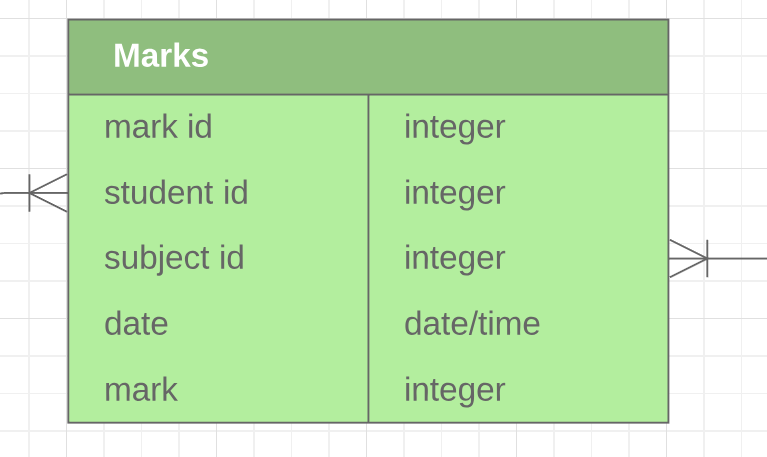
\includegraphics{01-img/1.png}
\caption{This is a entity.}
\end{figure}

My example is a table called \texttt{Marks}, which has
\texttt{mark\ id}, \texttt{student\ id}, \texttt{subject\ id},
\texttt{date} and \texttt{mark} as attributes. The other column is the
variable's type.

\subsubsection{Atributte}\label{atributte}

An attribute is a feature we want to keep track.

\subsubsection{Relationship}\label{relationship}

Is a way to connect two tables.

\begin{figure}
\centering
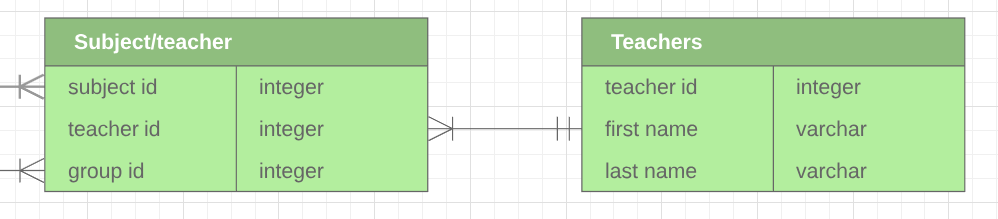
\includegraphics{01-img/2.png}
\caption{The line connecting two tables is a relationship.}
\end{figure}

Remember, this line has some properties, that is named as cardinality.

\subsubsection{Cardinality}\label{cardinality}

Cardinality represents a notation of how the information between tables
will interact with each other.

\begin{figure}
\centering
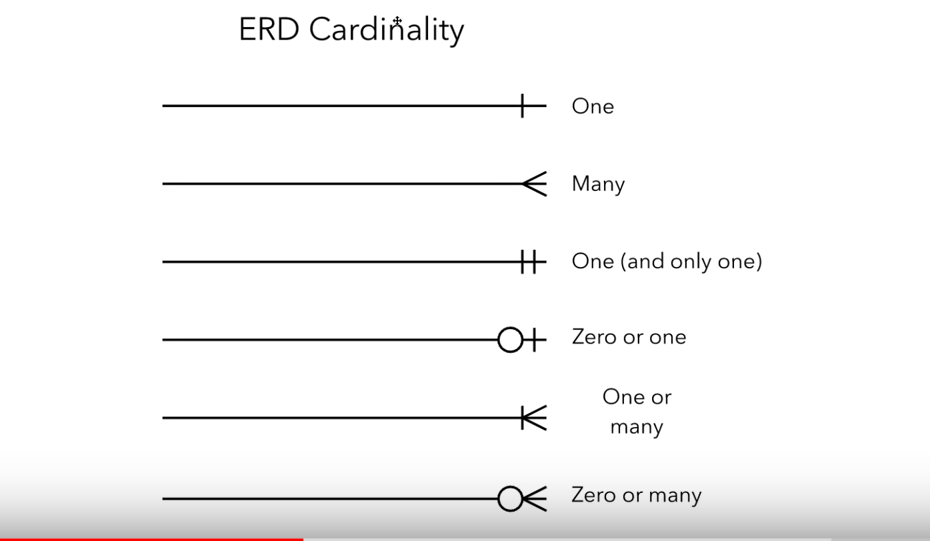
\includegraphics{01-img/3.png}
\caption{In a nutshell of Cardinality - Extracted from the Lucidchart
Video.}
\end{figure}

Additional videos with good content.

\href{https://www.youtube.com/watch?v=QpdhBUYk7Kk\&vl=en}{Video 1 -
Lucidchart} \href{https://www.youtube.com/watch?v=-CuY5ADwn24}{Vídeo 2 -
Lucidchart}

\begin{center}\rule{0.5\linewidth}{\linethickness}\end{center}

\subsection{SQL Introduction}\label{sql-introduction}

SQL is a Language used to manage this interactions between tables,
allowing us to access the stored database. The meaning of SQL is:

\begin{quote}
Structured Query Language
\end{quote}

It is very popular in Data Analysis because:

\begin{itemize}
\tightlist
\item
  Easy to understand
\item
  Easy to learn
\item
  Used to access very large datasets directly where is stored
\item
  Easy to audit and replicate
\item
  It is possible to run multiple queries at onde
\item
  Almost do not have a limit of rows/observations
\item
  Ensure the data Integrity, it is not possible to register a half child
  if you have defined this field as an integer
\item
  SQL is very fast
\item
  Database provide the data sharing, everybody could access the data
  simultaneously, which is good due to a standardization of database
\end{itemize}

SQL provides also functions such as:

\begin{itemize}
\tightlist
\item
  Summation
\item
  Count
\item
  Max and min
\item
  Mean, etc.
\end{itemize}

Have in mind, probably we are going to manipulate data, and rarely
updating or change values.

SQL is not case sensitive, so the best practices is to write the
clauses/staments in upper case.

\textbf{Best practices}

\begin{Shaded}
\begin{Highlighting}[]
\KeywordTok{SELECT}\NormalTok{ first_column}
  \KeywordTok{FROM}\NormalTok{ my_table}
\end{Highlighting}
\end{Shaded}

\textbf{Bad one}

\begin{Shaded}
\begin{Highlighting}[]
\KeywordTok{SelecT}\NormalTok{ first_column}
\KeywordTok{from}\NormalTok{ my_table}
\end{Highlighting}
\end{Shaded}

Bear in mind, the indentation is not a requirements but helps a lot to
understand your code.

\subsubsection{SQL vs.~NoSQL}\label{sql-vs.nosql}

Extracted from the class notes.

\begin{quote}
You may have heard of NoSQL, which stands for not only SQL. Databases
using NoSQL allow for you to write code that interacts with the data a
bit differently than what we will do in this course. These NoSQL
environments tend to be particularly popular for web based data, but
less popular for data that lives in spreadsheets the way we have been
analyzing data up to this point. One of the most popular NoSQL languages
is called MongoDB. Udacity has a full course on MongoDB that you can
take for free here, but these will not be a focus of this program. NoSQL
is not a focus of analyzing data in this Nanodegree program, but you
might see it referenced outside this course!
\end{quote}

\subsection{Clauses}\label{clauses}

Tell the database what to do.

\subsubsection{\texorpdfstring{\texttt{DROP\ TABLE}}{DROP TABLE}}\label{drop-table}

Remove a table from the database.

\subsubsection{\texorpdfstring{\texttt{CREATE\ TABLE}}{CREATE TABLE}}\label{create-table}

Create a new table.

\subsubsection{\texorpdfstring{\texttt{SELECT}}{SELECT}}\label{select}

Is also know as query, is used to create a new table with the selected
variables. You can use \texttt{*} if you want to select all columns.

\begin{Shaded}
\begin{Highlighting}[]
\KeywordTok{SELECT}\NormalTok{ first_column, second_column, last_column}
  \KeywordTok{FROM}\NormalTok{ first_table;}
\end{Highlighting}
\end{Shaded}

\subsubsection{\texorpdfstring{\texttt{LIMIT}}{LIMIT}}\label{limit}

This is the same of \texttt{.head()} but this could only load a few
lines to analyses the table.

\begin{Shaded}
\begin{Highlighting}[]
\KeywordTok{SELECT}\NormalTok{ first_column}
  \KeywordTok{FROM}\NormalTok{ my_table}
\KeywordTok{LIMIT} \DecValTok{1000}            \CommentTok{/* Will load the firs 1000 lines*/}
\end{Highlighting}
\end{Shaded}

\subsubsection{\texorpdfstring{\texttt{ORDER\ BY}}{ORDER BY}}\label{order-by}

It is possible to order by in ascendant and descendent way.

\textbf{ascendant}

\begin{Shaded}
\begin{Highlighting}[]
\KeywordTok{SELECT}\NormalTok{ first_column, second_column, last_column}
  \KeywordTok{FROM}\NormalTok{ my_table}
\KeywordTok{ORDER} \KeywordTok{BY}\NormalTok{ last_column }\CommentTok{/*ascendanting*/}
\KeywordTok{LIMIT} \DecValTok{1000}
\end{Highlighting}
\end{Shaded}

\textbf{descendent}

\begin{Shaded}
\begin{Highlighting}[]
\KeywordTok{SELECT}\NormalTok{ first_column, second_column, last_column}
  \KeywordTok{FROM}\NormalTok{ my_table}
\KeywordTok{ORDER} \KeywordTok{BY}\NormalTok{ last_column }\KeywordTok{DESC}\NormalTok{, second_column }\CommentTok{/*descending for last_column*/}
\KeywordTok{LIMIT} \DecValTok{1000}
\end{Highlighting}
\end{Shaded}

This last query will returns:

\begin{itemize}
\tightlist
\item
  Last\_column ordered by the highest to lowest;
\item
  The second\_column will be the lowest to highest.
\end{itemize}

\subsubsection{\texorpdfstring{\texttt{WHERE}}{WHERE}}\label{where}

Apply a filter to find a specific customer or anything else.

\begin{Shaded}
\begin{Highlighting}[]
\KeywordTok{SELECT}\NormalTok{ first_column, second_column, last_column}
  \KeywordTok{FROM}\NormalTok{ my_table}
\KeywordTok{WHERE}\NormalTok{ first_column = }\DecValTok{100}
\KeywordTok{ORDER} \KeywordTok{BY}\NormalTok{ second_column}
\KeywordTok{LIMIT} \DecValTok{100}
\end{Highlighting}
\end{Shaded}

All staments possible to use. * \texttt{\textgreater{}} (greater than) *
\texttt{\textless{}} (less than) * \texttt{\textgreater{}=} (greater
than or equal to) * \texttt{\textless{}=} (less than or equal to) *
\texttt{=} (equal to) * \texttt{!=} (not equal to)

If the argument of the WHERE clause is not a number, you must use single
quotes.

\begin{Shaded}
\begin{Highlighting}[]
\KeywordTok{SELECT}\NormalTok{ first_column, second_column, last_column}
  \KeywordTok{FROM}\NormalTok{ my_table}
\KeywordTok{WHERE}\NormalTok{ first_column = }\StringTok{'Hello World!'}
\KeywordTok{ORDER} \KeywordTok{BY}\NormalTok{ second_column}
\KeywordTok{LIMIT} \DecValTok{100}
\end{Highlighting}
\end{Shaded}

\subsection{Derived Columns}\label{derived-columns}

Is a new column created from the query. It is similar to the
\texttt{mutate} function from R.

This is the operator to create a derived column:

\begin{itemize}
\tightlist
\item
  \texttt{*} (Multiplication)
\item
  \texttt{+} (Addition)
\item
  \texttt{-} (Subtraction)
\item
  \texttt{/} (Division)
\end{itemize}

\begin{Shaded}
\begin{Highlighting}[]
\KeywordTok{SELECT} \KeywordTok{id}\NormalTok{, (standard_amt_usd/total_amt_usd)*}\DecValTok{100}
\KeywordTok{FROM}\NormalTok{ orders}
\KeywordTok{LIMIT} \DecValTok{10}\NormalTok{;}
\end{Highlighting}
\end{Shaded}

Will display without a specific name (?column?).

\subsubsection{\texorpdfstring{\texttt{AS}}{AS}}\label{as}

If you use the \texttt{AS} the derived column will be name as you define
(in other words ``alias'').

\begin{Shaded}
\begin{Highlighting}[]
\KeywordTok{SELECT} \KeywordTok{id}\NormalTok{, (standard_amt_usd/total_amt_usd)*}\DecValTok{100} \KeywordTok{AS}\NormalTok{ std_percent, total_amt_usd}
\KeywordTok{FROM}\NormalTok{ orders}
\KeywordTok{LIMIT} \DecValTok{10}\NormalTok{;}
\end{Highlighting}
\end{Shaded}

Best pratices: No capital letters, descriptive names, etc.

\subsection{\texorpdfstring{Introduction to ``Logical
Operators''}{Introduction to Logical Operators}}\label{introduction-to-logical-operators}

In the next concepts, you will be learning about Logical Operators.
Logical Operators include:

\subsubsection{LIKE}\label{like}

Using with WHERE clause could search some patterns.

\begin{Shaded}
\begin{Highlighting}[]
\KeywordTok{SELECT}\NormalTok{ first_column, second_column, last_column}
  \KeywordTok{FROM}\NormalTok{ my_table}
\KeywordTok{WHERE}\NormalTok{ last_column }\KeywordTok{LIKE} \StringTok{'%ello%'}
\end{Highlighting}
\end{Shaded}

The \texttt{\%} is called wild-card.

\subsubsection{IN}\label{in}

It is the same in Python or R. \texttt{IN} will be used to filter the
dataset based on a list.

\begin{Shaded}
\begin{Highlighting}[]
\KeywordTok{SELECT}\NormalTok{ first_column, second_column, last_column}
  \KeywordTok{FROM}\NormalTok{ my_table}
\KeywordTok{WHERE}\NormalTok{ last_column }\KeywordTok{IN}\NormalTok{ (}\DecValTok{100}\NormalTok{, }\DecValTok{200}\NormalTok{)}
\end{Highlighting}
\end{Shaded}

This example will filter the rows of last\_column with values of 100 or
200.

\subsubsection{NOT}\label{not}

\texttt{NOT} return the reverse/opposite.

\begin{Shaded}
\begin{Highlighting}[]
\KeywordTok{SELECT}\NormalTok{ first_column, second_column, last_column}
  \KeywordTok{FROM}\NormalTok{ my_table}
\KeywordTok{WHERE}\NormalTok{ last_column }\KeywordTok{NOT} \KeywordTok{IN}\NormalTok{ (}\DecValTok{100}\NormalTok{, }\DecValTok{200}\NormalTok{)}
\end{Highlighting}
\end{Shaded}

This example will remove all observations equals to 100 or 200.

Possible uses:

\begin{itemize}
\tightlist
\item
  NOT IN
\item
  NOT LIKE
\end{itemize}

\subsubsection{AND}\label{and}

Logical statment usually to make some filtration.

\begin{Shaded}
\begin{Highlighting}[]
\KeywordTok{SELECT}\NormalTok{ *}
\KeywordTok{FROM}\NormalTok{ orders}
\KeywordTok{WHERE}\NormalTok{ standard_qty > }\DecValTok{1000} \KeywordTok{AND}\NormalTok{ poster_qty = }\DecValTok{0} \KeywordTok{AND}\NormalTok{ gloss_qty = }\DecValTok{0}\NormalTok{;}
\end{Highlighting}
\end{Shaded}

\subsubsection{BETWEEN}\label{between}

Sometimes AND statment could be replaced by BETWEEN, this is much
clearly to understand. BUT the BETWEEN is inclusive, which means the
endpoints will be included in the filter.

\begin{Shaded}
\begin{Highlighting}[]
\KeywordTok{SELECT}\NormalTok{ name}
\KeywordTok{FROM}\NormalTok{ accounts}
\KeywordTok{WHERE}\NormalTok{ name }\KeywordTok{NOT} \KeywordTok{LIKE} \StringTok{'C%'} \KeywordTok{AND}\NormalTok{ name }\KeywordTok{LIKE} \StringTok{'%s'}\NormalTok{;}
\end{Highlighting}
\end{Shaded}

\subsubsection{OR}\label{or}

Well, this is a logical operator.

\begin{Shaded}
\begin{Highlighting}[]
\KeywordTok{SELECT} \KeywordTok{id}
\KeywordTok{FROM}\NormalTok{ orders}
\KeywordTok{WHERE}\NormalTok{ gloss_qty > }\DecValTok{4000} \KeywordTok{OR}\NormalTok{ poster_qty > }\DecValTok{4000}\NormalTok{;}
\end{Highlighting}
\end{Shaded}

\section{SQL Joins}\label{sql-joins}

\subsection{Joins}\label{joins}

When a table is splited the performance to update or just to make a
query is better than a big one. The reason is the quantity of data to
read. This is one of the reason to split dataset in several tables, even
more, sometimes in convinient to split because the type of data stored.

The reason of JOIN is to ``bind'' two datasets into one. Here we need to
use the period \texttt{.} (table.colums) to reference which
column/variable we want to select.

\begin{Shaded}
\begin{Highlighting}[]
\KeywordTok{SELECT}\NormalTok{ accounts.name, orders.occurred_at}
  \KeywordTok{FROM}\NormalTok{ orders}
\KeywordTok{JOIN}\NormalTok{ accounts}
\KeywordTok{ON}\NormalTok{ orders.account_id = accounts.id;}
\end{Highlighting}
\end{Shaded}

The result of this query is two columns (\texttt{name} and
\texttt{occured\_at}), and to linked by the \texttt{account\_id} and
\texttt{id}.

\subsubsection{Primary Key (PK)}\label{primary-key-pk}

Is a columns with unique values used to map a variable.

\subsubsection{Foreign Key (FK)}\label{foreign-key-fk}

Is a Primary Key from the other table. We use the PK and FK to link the
tables.

Based on the new information about \texttt{PK} and \texttt{FK}. Let's
insert a picture to visualize the database.

\begin{figure}
\centering
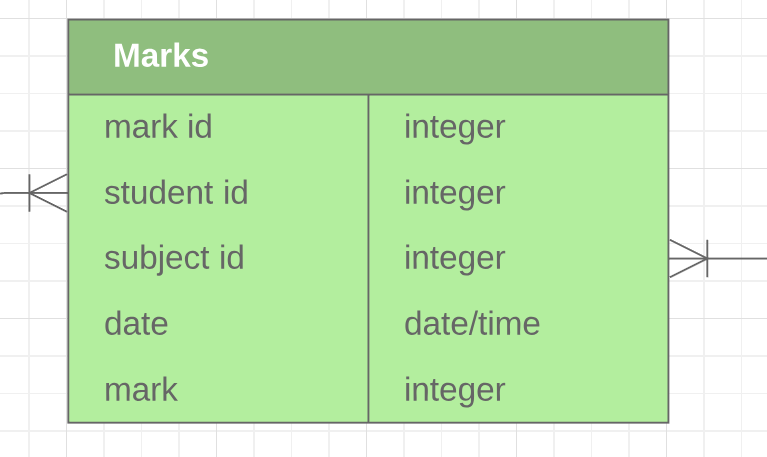
\includegraphics{01-img/1.png}
\caption{Example of Join}
\end{figure}

I want to Join these tables. My query:

\begin{Shaded}
\begin{Highlighting}[]
\KeywordTok{SELECT}\NormalTok{ orders.*}
\KeywordTok{FROM}\NormalTok{ orders}
\KeywordTok{JOIN}\NormalTok{ accounts}
\KeywordTok{ON}\NormalTok{ orders.account_id = accounts.id;}
\end{Highlighting}
\end{Shaded}

What I need to realize:

\begin{itemize}
\tightlist
\item
  \texttt{PK} and \texttt{FK} \textbf{always} will be allocated in
  \texttt{ON}.
\item
  \texttt{FROM} and \texttt{JOIN} each one with one table.
\end{itemize}

\subsubsection{Binding three tables}\label{binding-three-tables}

It is possible to ``chaining'' three tables.

\begin{Shaded}
\begin{Highlighting}[]
\KeywordTok{SELECT}\NormalTok{ *}
\KeywordTok{FROM}\NormalTok{ web_events}
\KeywordTok{JOIN}\NormalTok{ accounts}
\KeywordTok{ON}\NormalTok{ web_events.account_id = accounts.id}
\KeywordTok{JOIN}\NormalTok{ orders}
\KeywordTok{ON}\NormalTok{ accounts.id = orders.account_id}
\end{Highlighting}
\end{Shaded}

In this case, I will import all columns, but I may want few columns.

\begin{Shaded}
\begin{Highlighting}[]
\KeywordTok{SELECT}\NormalTok{ web_events.channel, accounts.name, orders.total}
\KeywordTok{FROM}\NormalTok{ web_events}
\KeywordTok{JOIN}\NormalTok{ accounts}
\KeywordTok{ON}\NormalTok{ web_events.account_id = accounts.id}
\KeywordTok{JOIN}\NormalTok{ orders}
\KeywordTok{ON}\NormalTok{ accounts.id = orders.account_id}
\end{Highlighting}
\end{Shaded}

\subsubsection{Alias}\label{alias}

Alias is a form to ``short'' the name of columns, the first method is
using \texttt{AS}, but it could be simplified by only a space.

\begin{itemize}
\tightlist
\item
  Example 1
\end{itemize}

\begin{Shaded}
\begin{Highlighting}[]
\KeywordTok{Select}\NormalTok{ t1.column1 aliasname, t2.column2 aliasname2}
\KeywordTok{FROM}\NormalTok{ tablename }\KeywordTok{AS}\NormalTok{ t1}
\KeywordTok{JOIN}\NormalTok{ tablename2 }\KeywordTok{AS}\NormalTok{ t2}
\end{Highlighting}
\end{Shaded}

\textbf{or}

\begin{Shaded}
\begin{Highlighting}[]
\KeywordTok{Select}\NormalTok{ t1.column1 aliasname, t2.column2 aliasname2}
\KeywordTok{FROM}\NormalTok{ tablename t1}
\KeywordTok{JOIN}\NormalTok{ tablename2 t2}
\end{Highlighting}
\end{Shaded}

\begin{itemize}
\tightlist
\item
  Example 2
\end{itemize}

\begin{Shaded}
\begin{Highlighting}[]
\KeywordTok{SELECT}\NormalTok{ col1 + col2 }\KeywordTok{AS}\NormalTok{ total, col3}
\end{Highlighting}
\end{Shaded}

\textbf{or}

\begin{Shaded}
\begin{Highlighting}[]
\KeywordTok{SELECT}\NormalTok{ col1 + col2 total, col3}
\end{Highlighting}
\end{Shaded}

\textbf{or}

\subsubsection{\texorpdfstring{\texttt{INNER\ JOIN}}{INNER JOIN}}\label{inner-join}

Returns rows which appears in both tables.

\begin{Shaded}
\begin{Highlighting}[]
\KeywordTok{SELECT}\NormalTok{ table_1.id, table_1.name, table_2.total}
  \KeywordTok{FROM}\NormalTok{ table_}\DecValTok{2}
    \KeywordTok{JOIN}\NormalTok{ table_}\DecValTok{1}
      \KeywordTok{ON}\NormalTok{ table_2.account_id = table_1.id}
\end{Highlighting}
\end{Shaded}

These last examples are all \texttt{INNER\ JOINS}, and will return a new
dataframe (intersection between two dataframes).

\subsubsection{\texorpdfstring{\texttt{OUTER\ JOIN}}{OUTER JOIN}}\label{outer-join}

There are two kinds of OUTER JOINs

\begin{itemize}
\tightlist
\item
  Left outer JOIN, and;
\item
  Right outer JOIN.
\end{itemize}

This two new JOINs has a property to pull rows that only exist in one
table, it means some rows might have NULL values. The standard for this
course will be to use only the left outer join.

\section{SQL Aggregations}\label{sql-aggregations}

\subsection{Aggregations Functions}\label{aggregations-functions}

This is functions return a single row with the aggregated value.

\begin{itemize}
\tightlist
\item
  sum;
\item
  min;
\item
  max;
\item
  mean, etc.
\end{itemize}

\subsubsection{NULL}\label{null}

NULL is no a value, it is different from ZERO or a space, for this
reason you can not use equal (\texttt{=}) to find it, for do so you must
use \texttt{IS}. The NULL is ignored in all aggregatins functions, and
it is defined as a property of the data.

For the \emph{Parch and Posey} dataset, NULL is equal to zero.

\begin{Shaded}
\begin{Highlighting}[]
\KeywordTok{WHERE}\NormalTok{ something }\KeywordTok{IS} \KeywordTok{NULL}
\KeywordTok{WHERE}\NormalTok{ something }\KeywordTok{IS} \KeywordTok{NOT} \KeywordTok{NULL}
\end{Highlighting}
\end{Shaded}

\paragraph{NULLs - Expert Tip}\label{nulls---expert-tip}

There are two common ways in which you are likely to encounter NULLs:

\begin{itemize}
\tightlist
\item
  NULLs frequently occur when performing a LEFT or RIGHT JOIN. You saw
  in the last lesson - when some rows in the left table of a left join
  are not matched with rows in the right table, those rows will contain
  some NULL values in the result set.
\item
  NULLs can also occur from simply missing data in our database.
\end{itemize}

\subsection{Functions}\label{functions}

\subsubsection{COUNT()}\label{count}

Count the number of rows. If the entire line has only NULLs, this line
will be noted counted.

Simple Example:

\begin{Shaded}
\begin{Highlighting}[]
\KeywordTok{SELECT} \FunctionTok{COUNT}\NormalTok{(*)}
\KeywordTok{FROM}\NormalTok{ accounts;}
\end{Highlighting}
\end{Shaded}

Example with filter

\begin{Shaded}
\begin{Highlighting}[]
\KeywordTok{SELECT} \FunctionTok{COUNT}\NormalTok{(*) }\KeywordTok{AS}\NormalTok{ order_count}
\KeywordTok{FROM}\NormalTok{ some_table}
\KeywordTok{WHERE}\NormalTok{ any_column > }\DecValTok{100} \KeywordTok{AND}\NormalTok{ any_column < }\DecValTok{200}\NormalTok{;}
\end{Highlighting}
\end{Shaded}

Example with column selection

\begin{Shaded}
\begin{Highlighting}[]
\KeywordTok{SELECT} \FunctionTok{COUNT}\NormalTok{(account.id)}
\KeywordTok{FROM}\NormalTok{ accounts;}
\end{Highlighting}
\end{Shaded}

\subsubsection{SUM()}\label{sum}

Perform the summation among rows. You must define which columns will be
applied the sum function.

\begin{Shaded}
\begin{Highlighting}[]
\KeywordTok{SELECT} \FunctionTok{SUM}\NormalTok{(poster_qty)}
\KeywordTok{FROM}\NormalTok{ demo.orders;}
\end{Highlighting}
\end{Shaded}

\subsubsection{MAX() and MIN()}\label{max-and-min}

Return a rows with the minimun or maximum of a given column.

\begin{Shaded}
\begin{Highlighting}[]
\KeywordTok{SELECT} \FunctionTok{MAX}\NormalTok{(poster_qty) }\KeywordTok{AS}\NormalTok{ max_poster_qty,}
       \FunctionTok{MIN}\NormalTok{(standard_qty) }\KeywordTok{AS}\NormalTok{ min_standard_qty}
\KeywordTok{FROM}\NormalTok{ demo.orders;}
\end{Highlighting}
\end{Shaded}

\subsubsection{GROUP BY}\label{group-by}

Divide the non-grouped column into groups, which means the aggregated
function will be calculated by group.

\begin{itemize}
\tightlist
\item
  The GROUP BY always goes between WHERE and ORDER BY.
\end{itemize}

Example 1:

\begin{Shaded}
\begin{Highlighting}[]
\KeywordTok{SELECT}\NormalTok{ a.name, o.occurred_at}
\KeywordTok{FROM}\NormalTok{ accounts a}
\KeywordTok{JOIN}\NormalTok{ orders o}
\KeywordTok{ON}\NormalTok{ a.id = o.account_id}
\KeywordTok{ORDER} \KeywordTok{BY}\NormalTok{ o.occurred_at}
\KeywordTok{LIMIT} \DecValTok{1}\NormalTok{;}
\end{Highlighting}
\end{Shaded}

Same example but indexing by number:

\begin{Shaded}
\begin{Highlighting}[]
\KeywordTok{SELECT}\NormalTok{ a.name, o.occurred_at}
\KeywordTok{FROM}\NormalTok{ accounts a}
\KeywordTok{JOIN}\NormalTok{ orders o}
\KeywordTok{ON}\NormalTok{ a.id = o.account_id}
\KeywordTok{ORDER} \KeywordTok{BY} \DecValTok{2}
\KeywordTok{LIMIT} \DecValTok{1}\NormalTok{;}
\end{Highlighting}
\end{Shaded}

\emph{OBS.: The index used in ORDER BY clause is to refence
o.occurred\_at.}

\subsubsection{DISTINCT}\label{distinct}

DISTINCT is always used in SELECT statements, and it provides the unique
rows for all columns written in the SELECT statement. Therefore, you
only use DISTINCT once in any particular SELECT statement.

\begin{Shaded}
\begin{Highlighting}[]
\KeywordTok{SELECT} \KeywordTok{DISTINCT}\NormalTok{ column1, column2, column3}
\KeywordTok{FROM}\NormalTok{ table1;}
\end{Highlighting}
\end{Shaded}

\subsubsection{HAVING}\label{having}

\begin{quote}
HAVING is the ``clean'' way to filter a query that has been aggregated,
but this is also commonly done using a subquery. Essentially, any time
you want to perform a WHERE on an element of your query that was created
by an aggregate, you need to use HAVING instead.
\end{quote}

Note extracted from the class notes.

\begin{Shaded}
\begin{Highlighting}[]
\KeywordTok{SELECT}\NormalTok{ s.id, s.name, }\FunctionTok{COUNT}\NormalTok{(*) num_accounts}
\KeywordTok{FROM}\NormalTok{ accounts a}
\KeywordTok{JOIN}\NormalTok{ sales_reps s}
\KeywordTok{ON}\NormalTok{ s.id = a.sales_rep_id}
\KeywordTok{GROUP} \KeywordTok{BY}\NormalTok{ s.id, s.name}
\KeywordTok{HAVING} \FunctionTok{COUNT}\NormalTok{(*) > }\DecValTok{5}
\KeywordTok{ORDER} \KeywordTok{BY}\NormalTok{ num_accounts;}
\end{Highlighting}
\end{Shaded}

\subsection{DATE}\label{date}

To GROUP BY a date is quite complicated because each time is (obviously)
different, for this, reason is necessary to ``round'' the time/date to
group them.

\subsubsection{DATE\_TRUNC}\label{date_trunc}

Common trunctions are:

\begin{itemize}
\tightlist
\item
  day;
\item
  month, and;
\item
  year.
\end{itemize}

Sintaxe:

DATE\_TRUNC(`{[}interval{]}', time\_column)

Where:

\begin{itemize}
\tightlist
\item
  microsecond
\item
  millisecond
\item
  second
\item
  minute
\item
  hour
\item
  day
\item
  week
\item
  month
\item
  quarter
\item
  year
\item
  century
\item
  decade
\item
  millenium
\end{itemize}

For further explanaition about
\href{https://blog.modeanalytics.com/date-trunc-sql-timestamp-function-count-on/}{date}

\begin{Shaded}
\begin{Highlighting}[]
\KeywordTok{SELECT}\NormalTok{ demo.accounts.name,}
\NormalTok{       DATE_TRUNC(}\StringTok{'month'}\NormalTok{, demo.orders.occurred_at) }\KeywordTok{AS}\NormalTok{ year_month,}
       \FunctionTok{SUM}\NormalTok{(demo.orders.gloss_amt_usd) }\KeywordTok{AS}\NormalTok{ sum_gloss_usd}
\KeywordTok{FROM}\NormalTok{ demo.orders}
\KeywordTok{JOIN}\NormalTok{ demo.accounts}
\KeywordTok{ON}\NormalTok{ demo.orders.account_id = demo.accounts.id}
\KeywordTok{WHERE}\NormalTok{ demo.accounts.name = }\StringTok{'Walmart'}
\KeywordTok{GROUP} \KeywordTok{BY}\NormalTok{ year_month, demo.accounts.name}
\KeywordTok{ORDER} \KeywordTok{BY}\NormalTok{ sum_gloss_usd }\KeywordTok{DESC}
\KeywordTok{LIMIT} \DecValTok{1}\NormalTok{;}
\end{Highlighting}
\end{Shaded}

\subsubsection{DATE PART}\label{date-part}

Extract part of the date

\subsection{CASE}\label{case}

Create a new column, derivate column, with a kind classification (assign
a value into this new column according to the statment).

\begin{Shaded}
\begin{Highlighting}[]
\KeywordTok{SELECT}\NormalTok{ account_id,}
\NormalTok{       occurred_at,}
\NormalTok{       total,}
       \KeywordTok{CASE} \KeywordTok{WHEN}\NormalTok{ total > }\DecValTok{500} \KeywordTok{THEN} \StringTok{'Over 500'}
            \KeywordTok{WHEN}\NormalTok{ total > }\DecValTok{300} \KeywordTok{AND}\NormalTok{ total <= }\DecValTok{500} \KeywordTok{THEN} \StringTok{'301 - 500'}
            \KeywordTok{WHEN}\NormalTok{ total > }\DecValTok{100} \KeywordTok{AND}\NormalTok{ total <= }\DecValTok{300} \KeywordTok{THEN} \StringTok{'101 - 300'}
            \KeywordTok{ELSE} \StringTok{'100 or under'} \KeywordTok{END} \KeywordTok{AS}\NormalTok{ total_group}
\KeywordTok{FROM}\NormalTok{ demo.orders}
\KeywordTok{LIMIT} \DecValTok{10}\NormalTok{;}
\end{Highlighting}
\end{Shaded}

Creates the total\_group column.

\subsubsection{With AGGREGATION}\label{with-aggregation}

Combining the CASE clause with aggregations function could be a power
tool, because the WHERE clause only evaluate one statement, using WHEN
CASE it is possible to evaluate several staments.

\begin{Shaded}
\begin{Highlighting}[]
\KeywordTok{SELECT}\NormalTok{ demo.orders.account_id,}
\NormalTok{       demo.orders.total_amt_usd,}
       \KeywordTok{CASE} \KeywordTok{WHEN}\NormalTok{ demo.orders.total_amt_usd >= }\DecValTok{3000} \KeywordTok{THEN} \StringTok{'Large'}
            \KeywordTok{ELSE} \StringTok{'Small'} \KeywordTok{END} \KeywordTok{AS} \KeywordTok{level}
\KeywordTok{FROM}\NormalTok{ demo.orders}
\KeywordTok{LIMIT} \DecValTok{10}\NormalTok{;}
\end{Highlighting}
\end{Shaded}

\section{SQL Subqueries \& Temporary Tables
(Advanced)}\label{sql-subqueries-temporary-tables-advanced}

\subsection{Subqueries}\label{subqueries}

This is a way to nest queries, it means: The result of one query will be
used as FROM to the next query.

\begin{Shaded}
\begin{Highlighting}[]
\KeywordTok{SELECT}\NormalTok{ *}
\KeywordTok{FROM}\NormalTok{(}\KeywordTok{SELECT}\NormalTok{ something}
     \KeywordTok{FROM}\NormalTok{   interesting) }\KeywordTok{AS}\NormalTok{ table_}\DecValTok{1}
\end{Highlighting}
\end{Shaded}

In the example above, I have one query nested to another. Bear in mind,
I must give a alias to the nested query.

If the result of the subquery is a single value, you are allowed to
insert this subquery wherever you want.

\subsection{WITH}\label{with}

Also known as \emph{Common Table Expression} (CTE), is a kinf of
subquery but could be more helpful if someone is going to read the code.
Due to the possibility to write the code in fragments an assign name,
this is very handy.

\textbf{Example}

\begin{Shaded}
\begin{Highlighting}[]
\KeywordTok{WITH}\NormalTok{ my_with_example }\KeywordTok{AS}\NormalTok{ (}\KeywordTok{SELECT}\NormalTok{ ... MY CODE)}

\KeywordTok{SELECT}\NormalTok{ something}
\KeywordTok{FROM}\NormalTok{ my_with_example}
\end{Highlighting}
\end{Shaded}

As you can see it provide a better way to code because the code became
more readable.

\section{Data Cleaning (Advanced)}\label{data-cleaning-advanced}

\subsection{Data Cleaning}\label{data-cleaning}

\subsubsection{LEFT and RIGHT}\label{left-and-right}

It is the same of Excel functions.

\begin{Shaded}
\begin{Highlighting}[]
\KeywordTok{SELECT} \KeywordTok{LEFT}\NormalTok{(}\DecValTok{2}\NormalTok{, something) }\KeywordTok{AS}\NormalTok{ lefty_part_of_simething}
\KeywordTok{FROM}\NormalTok{ interesting}
\end{Highlighting}
\end{Shaded}

The example above will create a new column with the first two, from the
left to right, character of something.

\begin{Shaded}
\begin{Highlighting}[]
\KeywordTok{SELECT} \KeywordTok{RIGHT}\NormalTok{(}\DecValTok{2}\NormalTok{, something) }\KeywordTok{AS}\NormalTok{ lefty_part_of_simething}
\KeywordTok{FROM}\NormalTok{ interesting}
\end{Highlighting}
\end{Shaded}

Almost the same, but start from the right to the left.

\subsubsection{LEN}\label{len}

Returns the string length.

\begin{Shaded}
\begin{Highlighting}[]
\KeywordTok{SELECT}\NormalTok{ LEN(something)}
\KeywordTok{FROM}\NormalTok{ interesting}
\end{Highlighting}
\end{Shaded}

\subsubsection{POSITION and STRPOS}\label{position-and-strpos}

POSITION will find a pattern in the string and will return the position
(from the left to the right).

\begin{Shaded}
\begin{Highlighting}[]
\KeywordTok{SELECT}\NormalTok{ POSITION(}\StringTok{','}\NormalTok{, something) }\CommentTok{/*Looking for a coma*/}
\KeywordTok{FROM}\NormalTok{ interesting}
\end{Highlighting}
\end{Shaded}

The STRPOS has the same use and same results.

\begin{Shaded}
\begin{Highlighting}[]
\KeywordTok{SELECT}\NormalTok{ STRPOS(something, }\StringTok{','}\NormalTok{) }\CommentTok{/*Looking for a coma*/}
\KeywordTok{FROM}\NormalTok{ interesting}
\end{Highlighting}
\end{Shaded}

Both functions are case sensitive.

\subsubsection{LOWER and UPPER}\label{lower-and-upper}

Converts string into all lower or all upper cases.

\begin{Shaded}
\begin{Highlighting}[]
\KeywordTok{SELECT} \FunctionTok{LOWER}\NormalTok{(something)}
\KeywordTok{FROM}\NormalTok{ interesting}
\end{Highlighting}
\end{Shaded}

\subsubsection{CONCAT}\label{concat}

Bind/Combine/Concatenate strings (in different) columns into a new
column.

\textbf{Example 1}

\begin{Shaded}
\begin{Highlighting}[]
\KeywordTok{SELECT} \FunctionTok{CONCAT}\NormalTok{(first_name, }\StringTok{' '}\NormalTok{,last_name) }\KeywordTok{AS}\NormalTok{ complete_name }\CommentTok{/* The ' ' is the space between strings*/}
\KeywordTok{FROM}\NormalTok{ interesting}
\end{Highlighting}
\end{Shaded}

You can use \textbar{}\textbar{}.

\textbf{Example 2}

\begin{Shaded}
\begin{Highlighting}[]
\KeywordTok{SELECT}\NormalTok{ first_name || }\StringTok{' '}\NormalTok{ || last_name }\KeywordTok{AS}\NormalTok{ complete_name }\CommentTok{/* The ' ' is the space between strings*/}
\KeywordTok{FROM}\NormalTok{ interesting}
\end{Highlighting}
\end{Shaded}

\subsubsection{CAST}\label{cast}

CAST allow to convert one type to another.

\textbf{Example 1}

\begin{Shaded}
\begin{Highlighting}[]
\KeywordTok{SELECT} \FunctionTok{CAST}\NormalTok{(}\DataTypeTok{year}\NormalTok{ || }\DataTypeTok{month}\NormalTok{ || }\DataTypeTok{day} \KeywordTok{AS} \DataTypeTok{date}\NormalTok{) }\KeywordTok{AS}\NormalTok{ formatted_date}
\KeywordTok{FROM}\NormalTok{ interesting}
\end{Highlighting}
\end{Shaded}

The same of Example 1, but with a different notation to CAST clause.

\textbf{Example 2:}

\begin{Shaded}
\begin{Highlighting}[]
\KeywordTok{SELECT}\NormalTok{ (}\DataTypeTok{year}\NormalTok{ || }\DataTypeTok{month}\NormalTok{ || }\DataTypeTok{day} \KeywordTok{AS} \DataTypeTok{date}\NormalTok{):}\CharTok{:date} \KeywordTok{AS}\NormalTok{ formatted_date}
\KeywordTok{FROM}\NormalTok{ interesting}
\end{Highlighting}
\end{Shaded}

CAST is useful to converter strings into numbers or dates.

\subsubsection{COALESCE}\label{coalesce}

Converts NULL fields into Zero.

\section{Project 01 - Chinook}\label{project-01---chinook}

Questions

All exercises of this chapter I have stored in the Mode Analytics
platform.

\href{https://modeanalytics.com/ah_uyekita/reports/5e871f63f8b2}{Optional
Questions}

Project Submitted

I have written all the project in Mode Analytics because is a better
place to coding.

\begin{itemize}
\tightlist
\item
  I can perform SQL queries;
\item
  I can create graphics;
\item
  An opportunity to get knowledge in a new tool.
\end{itemize}

\href{https://modeanalytics.com/ah_uyekita/reports/e77643786160}{Project
01 in Mode Analytic}

\begin{center}\rule{0.5\linewidth}{\linethickness}\end{center}

\subsection{Project Submission}\label{project-submission}

To submit your project, please do the following:

\begin{itemize}
\tightlist
\item
  Review your project against the project Rubric. Reviewers will use
  this to evaluate your work.
\item
  Create your slides with whatever presentation software you'd like
  (e.g.~Google Slides, PowerPoint, Keynote, etc.).
\end{itemize}

In order to review your presentation, you will need to save your slides
as a PDF. You can do this from within Google Slides by selecting File
\textgreater{} Download as \textgreater{} PDF Document.

\begin{center}\rule{0.5\linewidth}{\linethickness}\end{center}

\chapter{Data Wrangling}\label{data-wrangling}

\section{Introduction to Data
Wrangling}\label{introduction-to-data-wrangling}

There are roughly three steps in the Data Wrangling.

\begin{itemize}
\tightlist
\item
  Gathering;
\item
  Assessing, and;
\item
  Cleaning.
\end{itemize}

This is a iterate process between these three steps.

\begin{quote}
Data wrangling is about gathering the right pieces of data, assessing
your data's quality and structure, then modifying your data to make it
clean. But the assessments you make and convert to cleaning operations
won't make your analysis, viz, or model better, though. The goal is to
just make them possible, i.e., functional.
\end{quote}

\begin{quote}
EDA is about exploring your data to later augment it to maximize the
potential of our analyses, visualizations, and models. When exploring,
simple visualizations are often used to summarize your data's main
characteristics. From there you can do things like remove outliers and
create new and more descriptive features from existing data, also known
as feature engineering. Or detect and remove outliers so your model's
fit is better.
\end{quote}

\begin{quote}
ETL: You also may have heard of the extract-transform-load process also
known as ETL. ETL differs from data wrangling in three main ways: * The
users are different * The data is different * The use cases are
different This article (Data Wrangling Versus ETL: What's the
Difference?) by Wei Zhang explains these three differences well.
\end{quote}

All text extracted from the class notes.

\subsection{Gathering}\label{gathering}

Gathering is the first step of a Data Wrangling, is also known as
Collecting or Acquiring. The Armenian Online Job Post has 19,000 jobs
postings from 2004 to 2015.

\begin{quote}
Best Practice: Downloading Files Programmatically
\end{quote}

This is the reasons:

\begin{itemize}
\tightlist
\item
  Scalability: This automation will save time, and prevents erros;
\item
  Reproducibility: Key point to any research. Anyone could reproduce
  your work and check it.
\end{itemize}

\subsection{Assessing}\label{assessing}

The assessing in divided into two mains aspects:

\begin{itemize}
\tightlist
\item
  Quality of the dataset
\item
  Tidiness of the dataset
\end{itemize}

\subsubsection{Quality}\label{quality}

Low quality dataset is related to a dirty dataset, which means the
content quality of data.

Commom issues:

\begin{itemize}
\tightlist
\item
  Missing values
\item
  Non standard units (km, meters, inches, etc. all mixed)
\item
  Innacurate data, invalid data, inconsistent data, etc.
\end{itemize}

\begin{quote}
One dataset may be high enough quality for one application but not for
another.
\end{quote}

\subsubsection{Tidiness}\label{tidiness}

Untidy data or \emph{messy} data, is about the structure of the dataset.

\begin{itemize}
\tightlist
\item
  Each obsevation by rows, and;
\item
  Each variable/features by column.
\end{itemize}

This is the Hadley Wickham definition of tidy data.

\subsection{Assessing the data}\label{assessing-the-data}

There are two ways to assess the data.

\begin{itemize}
\tightlist
\item
  Visual, and;
\item
  Programmatic.
\end{itemize}

\subsubsection{Visual Assessment}\label{visual-assessment}

Using regular tools, such as Graphics, Excel, tables, etc. It means,
there is a human assessing the data.

\subsubsection{Programmatic Assessment}\label{programmatic-assessment}

Using automation to dataset evaluation is scalable, and allows you to
handle a very huge quantity of data.

Examples of ``Programmatic Assessment'': Analysing the data using
\texttt{.info()}, \texttt{.head()}, \texttt{.describe()}, plotting
graphics (\texttt{.plot()}), etc..

Bear in mind, in this step we do not use ``verbs'' to describe any
erros/problem, because the ``verbs'' will be actions to the next step.

\subsection{Cleaning}\label{cleaning}

Improving the quality of a dataset or cleaning the dataset do not means:
Changing the data (because it could be \textbf{data fraud}).

The meaning of Cleaning is correcting the data or removing the data.

\begin{itemize}
\tightlist
\item
  Innacurate, wrong or irrelevant data.
\item
  Replacing or filling (NULL or NA values) data.
\item
  Combining/Merging datasets.
\end{itemize}

Improving the tidiness is transform the dataset to follow:

\begin{itemize}
\tightlist
\item
  each observation = row
\item
  each variable = column
\end{itemize}

There are two ways to cleaning the data: manually and programmatic.

\subsubsection{Manually}\label{manually}

To be avoided.

\subsubsection{Programmatic}\label{programmatic}

There are three steps:

\begin{enumerate}
\def\labelenumi{\arabic{enumi}.}
\tightlist
\item
  Define
\item
  Code
\item
  Test
\end{enumerate}

\begin{quote}
\textbf{Defining} means defining a data cleaning plan in writing, where
we turn our assessments into defined cleaning tasks. This plan will also
serve as an instruction list so others (or us in the future) can look at
our work and reproduce it.
\end{quote}

\begin{quote}
\textbf{Coding} means translating these definitions to code and
executing that code.
\end{quote}

\begin{quote}
\textbf{Testing} means testing our dataset, often using code, to make
sure our cleaning operations worked.
\end{quote}

Text from the class notes.

\section{Data Gathering}\label{data-gathering}

This is the first step of any Data Wrangling, sometimes this process is
a bit complicated because you need to find these data (probably from
different sources and then merge).

\subsection{Flat File}\label{flat-file}

This is the way to store data into a single text file, usually, this
file has another extension (.csv, tsv, etc.), each one of this extension
has your own characteristic.

\begin{itemize}
\tightlist
\item
  Each variable/features is separated by a comma and each row is an
  observation;
\item
  Each variable/features is separated by a tab and each row is an
  observation.
\end{itemize}

There are some \textbf{advantages} for using the flat files.

\begin{itemize}
\tightlist
\item
  Anyone could read, even a human;
\item
  Is lightweight;
\item
  You do not need to install a specific software;
\item
  Simple to understand (each variable is delimited by a coma/tab);
\item
  Any software could open it;
\item
  Very good to small dataset.
\end{itemize}

But has disadvantages also:

\begin{itemize}
\tightlist
\item
  Do not have standard;
\item
  Do not have data integrity checks;

  \begin{itemize}
  \tightlist
  \item
    Duplicated rows;
  \item
    You can record any value in any field;
  \end{itemize}
\item
  Not great to large datasets.
\end{itemize}

\paragraph{Importing the tsv file}\label{importing-the-tsv-file}

I have used the \texttt{read\_csv} to load the data, but I have set the
sep argument as \texttt{\textbackslash{}t}, which means tabular.
Sometimes, the flat files use \texttt{;} or \texttt{,}, so it is
necessary to define what is the delimiter.

\textbf{Example:}

\begin{Shaded}
\begin{Highlighting}[]
\ImportTok{import}\NormalTok{ pandas }\ImportTok{as}\NormalTok{ pd}
\NormalTok{df }\OperatorTok{=}\NormalTok{ pd.read_cvs(}\StringTok{'bestofrt.tsv'}\NormalTok{, sep}\OperatorTok{=} \StringTok{'}\CharTok{\textbackslash{}t}\StringTok{'}\NormalTok{)}
\end{Highlighting}
\end{Shaded}

\subsection{Web Scraping}\label{web-scraping}

This is terminology is used to say the data extracted from a website
(usually using code to do it). Due to this code depends on the HTML
file, if any change of the website happens, all the code used to web
scrapping could stopping to working properly, which requires an
adjustments. For this reason, web scraping is not a definitive solution.

\subsection{HTTP Request}\label{http-request}

This is useful to access archives from the internet, combining with the
OS package, it is possible to download and store locally the file.

\subsection{Encoding and Character
Set}\label{encoding-and-character-set}

This explanation is based on
\href{https://stackoverflow.com/questions/6224052/what-is-the-difference-between-a-string-and-a-byte-string}{this}
Stack Overflow thread.

Encoding: Is a proccess to convert a something into bytes.

\begin{itemize}
\tightlist
\item
  Audio is encoded into MP3, WAV, etc.
\item
  Images is encoded into PNG, JPG, TIFF, etc.
\item
  Text files is enconded into ASCII, UTF-8, etc.
\end{itemize}

The Character Set is as the name, is a set of charaters which I can use
to write a phrase, each character has a code which represents the
letter/character. There are several character set such as ASCII and
UTF-8.

\subsection{Application Programming Interfaces -
API}\label{application-programming-interfaces---api}

The API let you access the data from the internet in a resonable easy
manner.

There are several API available in the internet for many social media:

\begin{itemize}
\tightlist
\item
  Facebook;
\item
  Instagram;
\item
  Twitter, etc.;
\end{itemize}

This lesson will use the
\href{https://www.mediawiki.org/wiki/MediaWiki}{Mediawiki}, which is a
Open Source API to Wikipedia.

Most of the file from the API are formated as JSON or XML.

\subsection{JSON and XML}\label{json-and-xml}

JSON stands for Javascript Object Notation and XML for Extensible Markup
Language.

Sometimes the regular tabular way to structure the data is not a good
solution, and for this reason, there are other forms to store data as
JSON and XML.

They use a kind of ``dictionary'' to store data, which allows storing
more than one information per variable.

There are some similarities in JSON and Python:

\begin{itemize}
\tightlist
\item
  JSON Array = Python list
\item
  JSON Object = Python dictonary
\end{itemize}

\subsection{Methods in this Lesson}\label{methods-in-this-lesson}

\subsubsection{\texorpdfstring{\texttt{.find()}}{.find()}}\label{find}

This method is used to find tags and containers.

\textbf{Example:}

\begin{Shaded}
\begin{Highlighting}[]
\NormalTok{soup.find(}\StringTok{'title'}\NormalTok{)}
\end{Highlighting}
\end{Shaded}

This code above will find the tag title, and return the content.

\subsubsection{\texorpdfstring{\texttt{.find\_all()}}{.find\_all()}}\label{find_all}

It is almost the same of \texttt{.find()}, but will find in all document
the given pattern.

\textbf{Example:}

\begin{Shaded}
\begin{Highlighting}[]
\NormalTok{something.find_all(}\StringTok{'div'}\NormalTok{)}
\end{Highlighting}
\end{Shaded}

This code will return all \texttt{div} in the document. It could be used
with \texttt{limit\ =\ 1}, which will return the first \texttt{div}.

\subsubsection{\texorpdfstring{\texttt{.contents}}{.contents}}\label{contents}

The \texttt{.contents} get the elements from the \texttt{find} and
\texttt{find\_all}.You are capable to select, which element you want
(indexing).

\begin{Shaded}
\begin{Highlighting}[]
\NormalTok{something.find_all(}\StringTok{'div'}\NormalTok{)[}\DecValTok{1}\NormalTok{].contents[}\DecValTok{2}\NormalTok{]}
\end{Highlighting}
\end{Shaded}

In this fragment of code, I am selecting only the third element of
\texttt{something.find\_all(\textquotesingle{}div\textquotesingle{}){[}1{]}}.

\subsubsection{\texorpdfstring{\texttt{os.listdir()}}{os.listdir()}}\label{os.listdir}

This function list all files inside a given folder/directory.

\begin{Shaded}
\begin{Highlighting}[]
\NormalTok{os.listdir(my_path)}
\end{Highlighting}
\end{Shaded}

\subsubsection{\texorpdfstring{\texttt{.glob()}}{.glob()}}\label{glob}

This method is a part of the glob package.

If you are familiar with Linux CLI, you have alread used the globbing to
find a file in a folder.

\begin{Shaded}
\begin{Highlighting}[]
\ImportTok{import}\NormalTok{ glob}
\NormalTok{glob.glob(}\StringTok{'any_folder/*.txt'}\NormalTok{)}
\end{Highlighting}
\end{Shaded}

The result of the \texttt{.glob()} will be a list with all files which
matches the \texttt{.txt}.

\subsubsection{\texorpdfstring{\texttt{.read()}}{.read()}}\label{read}

Convert the file into a in memory variable.

\begin{Shaded}
\begin{Highlighting}[]
\NormalTok{my_new_variable }\OperatorTok{=} \BuiltInTok{file}\NormalTok{.read() }\CommentTok{# my_new_variable is a variable which contains the file.}
\end{Highlighting}
\end{Shaded}

\subsubsection{\texorpdfstring{\texttt{.readline()}}{.readline()}}\label{readline}

Read line by line every instance which is used this method.

\begin{Shaded}
\begin{Highlighting}[]
\BuiltInTok{file}\NormalTok{.readline() }\CommentTok{# Read the first line of the document file}
\BuiltInTok{file}\NormalTok{.readline() }\CommentTok{# Read the second line of the document file}
\BuiltInTok{file}\NormalTok{.read()     }\CommentTok{# Read the rest of the content.}
\end{Highlighting}
\end{Shaded}

\subsubsection{\texorpdfstring{\texttt{.DataFrame()}}{.DataFrame()}}\label{dataframe}

This method from the pandas package converts a simple dictonary to a
Pandas DataFrame.

\begin{Shaded}
\begin{Highlighting}[]
\NormalTok{pd.DataFrame(my_dataframe, columns }\OperatorTok{=}\NormalTok{ [}\StringTok{'column_1'}\NormalTok{, }\StringTok{'column_2'}\NormalTok{, }\StringTok{'column_3'}\NormalTok{])}
\end{Highlighting}
\end{Shaded}

\subsubsection{\texorpdfstring{\texttt{.page()}}{.page()}}\label{page}

The \texttt{.page()} method from the wptools package converts a
Wikipedia page into a object.

\begin{Shaded}
\begin{Highlighting}[]
\NormalTok{any_website }\OperatorTok{=}\NormalTok{ wptools.page(}\StringTok{'E.T._the_Extra-Terrestrial'}\NormalTok{)}
\end{Highlighting}
\end{Shaded}

\subsubsection{\texorpdfstring{\texttt{.get()}}{.get()}}\label{get}

The \texttt{.get()} method from the wptools package extract all info
from the wptools object.

\begin{Shaded}
\begin{Highlighting}[]
\NormalTok{any_website }\OperatorTok{=}\NormalTok{ wptools.page(}\StringTok{'E.T._the_Extra-Terrestrial'}\NormalTok{).get()}
\end{Highlighting}
\end{Shaded}

\section{Assessing Data}\label{assessing-data}

This is the second step of the Data Wrangling, and the aims of this
lesson is to explain some details. There are two kind of \emph{unclean}
data:

\begin{itemize}
\tightlist
\item
  Quality issues: Dirty data;

  \begin{itemize}
  \tightlist
  \item
    Missing, duplicated, or incorrect data;
  \end{itemize}
\item
  Lack of tidiness: Also known as messy data.

  \begin{itemize}
  \tightlist
  \item
    Strucutural issues
  \end{itemize}
\end{itemize}

There are two ways to assess:

\begin{itemize}
\tightlist
\item
  Visual: Plotting a simple graphic or visualizing the table (rows and
  columns);
\item
  Programmatic: Using code to summarize the data frame using .info(),
  .describe(), average, summation, max, min, etc..
\end{itemize}

\subsubsection{Dirty Data}\label{dirty-data}

Is related to the content issues, as known as low quality data.

\begin{itemize}
\tightlist
\item
  Innacurated data: Typos, corrupted, and duplicated data;
\end{itemize}

\subsubsection{Messy Data}\label{messy-data}

Messy data is related to structural issues, as known as untidy data.

\begin{itemize}
\tightlist
\item
  Each observation is a row;
\item
  Each variable/features is a column;
\item
  Based on the Hadley Wickham principles of tidy data.
\end{itemize}

\subsection{Assess Proccess}\label{assess-proccess}

In both cases (visual or programmatic), we could be divided into two
main steps:

\begin{itemize}
\tightlist
\item
  Detect;
\item
  Document.
\end{itemize}

\subsection{Data Quality Dimensions}\label{data-quality-dimensions}

\begin{quote}
Data quality dimensions help guide your thought process while assessing
and also cleaning. The four main data quality dimensions are:
\end{quote}

\begin{itemize}
\tightlist
\item
  Completeness: Missing values;
\item
  Validity: Invalid value (like negative height or weight, zip code with
  only 4 digits, etc.);
\item
  Accuracy: Wrong data which is valid (like the typo in the height);
\item
  Consistency: Data without a standard notation (New York and NY,
  Colorado and CO, same information but differents notations).
\end{itemize}

The severity of this problem is decreasing order: Completeness,
Validity, Accuracy, and Consistency.

\section{Cleaning Data}\label{cleaning-data}

Always opt to clean the data using the Programmatic way because manually
it is more error prone.

This is the steps of Data Cleaning:

\begin{itemize}
\tightlist
\item
  Define: Defining a Data Cleaning Plan (usually writting down);
\item
  Code: Converts the Data Cleaning Plan into code;
\item
  Test: Evaluates the outuput of the code.
\end{itemize}

\subsection{Tidiness}\label{tidiness-1}

It is the standard preconized by Hadley Wickham.

Usually, the tidiness issues is the first to be solved.

\subsection{Quality}\label{quality-1}

After fixing tidiness issues, the quality issues could be fixed.

\subsection{Methods}\label{methods}

\subsubsection{\texorpdfstring{\texttt{.melt()}}{.melt()}}\label{melt}

Convert a wide format to a long format. It is the same of gather and
spread functions from tidyr R package.

\href{https://www.youtube.com/watch?v=qOkj5zOHwRE}{Good Video -
Explaning the melt}

\section{Project 02 - Wrangle and Analyze
Data}\label{project-02---wrangle-and-analyze-data}

Project Submitted

Please, find below the URL to redirect to the project Jupyter Notebook.

\href{https://github.com/AndersonUyekita/ND111_data_science_foundations_02/blob/master/03-Chapter03/00-Project_02/wrangle_act.ipynb}{Project
02 - WeRateDogs™ - Wrangle and Analyze Data}

\begin{center}\rule{0.5\linewidth}{\linethickness}\end{center}

\subsection{Project Submission}\label{project-submission-1}

In this project, you'll gather, assess, and clean data then act on it
through analysis, visualization and/or modeling.

Before you submit:

\begin{enumerate}
\def\labelenumi{\arabic{enumi}.}
\item
  Ensure you meet specifications for all items in the Project Rubric.
  Your project ``meets specifications'' only if it meets specifications
  for all of the criteria.
\item
  Ensure you have not included your API keys, secrets, and tokens in
  your project files.
\item
  If you completed your project in the Project Workspace, ensure the
  following files are present in your workspace, then click ``Submit
  Project'' in the bottom righthand corner of the Project Workspace
  page:
\end{enumerate}

\begin{itemize}
\tightlist
\item
  \texttt{wrangle\_act.ipynb}: code for gathering, assessing, cleaning,
  analyzing, and visualizing data
\item
  \texttt{wrangle\_report.pdf} or wrangle\_report.html: documentation
  for data wrangling steps: gather, assess, and clean
\item
  \texttt{act\_report.pdf} or \texttt{act\_report.html}: documentation
  of analysis and insights into final data
\item
  \texttt{twitter\_archive\_enhanced.csv}: file as given
\item
  \texttt{image\_predictions.tsv}: file downloaded programmatically
\item
  \texttt{tweet\_json.txt}: file constructed via API
\item
  \texttt{twitter\_archive\_master.csv}: combined and cleaned data
\item
  any additional files (e.g.~files for additional pieces of gathered
  data or a database file for your stored clean data)
\end{itemize}

\begin{enumerate}
\def\labelenumi{\arabic{enumi}.}
\setcounter{enumi}{3}
\tightlist
\item
  If you completed your project outside of the Udacity Classroom,
  package the above listed files into a zip archive or push them from a
  GitHub repo, then click the ``Submit Project'' button on this page.
\end{enumerate}

As stated in point 4 above, you can submit your files as a zip archive
or you can link to a GitHub repository containing your project files. If
you go with GitHub, note that your submission will be a snapshot of the
linked repository at time of submission. It is recommended that you keep
each project in a separate repository to avoid any potential confusion:
if a reviewer gets multiple folders representing multiple projects,
there might be confusion regarding what project is to be evaluated.

It can take us up to a week to grade the project, but in most cases it
is much faster. You will get an email once your submission has been
reviewed. If you are having any problems submitting your project or wish
to check on the status of your submission, please email us at
\href{mailto:review-support@udacity.com}{\nolinkurl{review-support@udacity.com}}.
In the meantime, you should feel free to proceed with your learning
journey by continuing on to the next module in the program.

\chapter{Applications}\label{applications}

Some \emph{significant} applications are demonstrated in this chapter.

\section{Example one}\label{example-one}

\section{Example two}\label{example-two}

\chapter{Intro to Machine Learning}\label{intro-to-machine-learning}

We have finished a nice book.

\chapter{Data Visualization
(Optional)}\label{data-visualization-optional}

We have finished a nice book.

\bibliography{book.bib,packages.bib}


\end{document}
